%%%%%%%%%%%%%%%%%%%%%%%%%%%%%%%%%%%%%%%%%%%%%%
\chapter{Optimization and commissioning for LHC Run 2}\label{ch:BPixCalib}
%%%%%%%%%%%%%%%%%%%%%%%%%%%%%%%%%%%%%%%%%%%%%%

The CMS pixel detector was designed to cope with the high radiation environment of LHC and to operate with the highest performance even after the accumulation of significant radiation doses.
Nevertheless, radiation damage affects hit efficiency and resolution and hence, it is necessary to monitor its effects during operations.
As described in this chapter, throughout Run~1, re-calibrations of the detector have been performed to compensate for these effects and recover full performance.

During LS1, both BPix and FPix were extracted from CMS for maintenance with the purpose to recover broken channels.
In this period, the calibration procedure has been exercized and improved in view of commissioning and operations for Run~2.

The pixel detector has been operated with a coolant temperature of 7.4\unit{$^\circ$C} in 2008--2011 and 0\unit{$^\circ$C} in 2012, which for the pixel sensors translates to values $\sim10$\unit{$^\circ$C} higher.
In order to limit the impact of radiation damage, during Run~2 the detector has been operated at much lower temperature, down to -10\unit{$^\circ$C}.
This has been made possible thanks to a major effort during the long shutdown to improve the sealing, insulation of the tracker detectors and also to upgrade the C$_6$F$_{14}$ cooling and dry gas plants.
During LS1, the pixel detector functionalities at very low temperature have been checked and its (temperature dependent) settings re-calibrated to allow for optimal operations under such conditions.
This activities, described in the following, have been crucial to allow for a quick and smooth re-installation and commissioning for Run~2, as well as for stable and excellent operations during 2015 and 2016.

%%%%%%%%%%%
\section{Effects of radiation damage in LHC Run 1}
%%%%%%%%%%%

One of the first visible effect of radiation is the increase of the sensor leakage current with integrated luminosity, due to damages in the silicon bulk.
The most fundamental type of bulk radiation damage is a defect, produced by the displacement of an atom of the semiconductor material from its normal lattice site.
The vacancy left behind, together with the original atom now at an interstitial position, constitutes a trapping site for normal charge carriers.
The formation of mid-gap states facilitates the transition of electrons from the valence to the conduction band leading to an increase of the leakage current in the depletion region.
The primary defects caused by irradiation are not stable but able to move through the crystal. As result of this diffusion process, there is the possibility of combination of more complex defects.
The whole process is called annealing with a beneficial part reducing the damage and a reverse one degrading macroscopic sensor properties, called ``reverse annealing''.
During beneficial annealing, with a time constant of a few days at room temperature, the leakage current decreases, while later it rises due to reverse annealing process until it finally saturates at a value which is significantly above the initial level. At temperatures below 0\unit{$^\circ$C} however, both effects can be frozen, so the detector current remains constant.
Thus, irradiated detectors in general should be operated and stored at low temperature, while it is favourable to shortly expose them to room temperature to take advantage of the beneficial annealing.

Figure~\ref{fig:PixLeakageCurrent} shows the increase of the leakage current during Run~1 for the pixel barrel layers measured from readings of the high voltage power supplies as a function of the integrated luminosity.
The damage was only partially recovered by beneficial annealing that took place during a longer shutdown after about 6\fbinv and a shorter technical stop after about 13\fbinv delivered integrated luminosity.
%The aforementioned diffusion processes in the silicon bulk are naturally temperature dependent and some effects can be frozen out at temperatures below 0\unit{$^\circ$C}.
Between the end of 2011 and the beginning of 2012 the operating temperature was decreased from 7.4\unit{$^\circ$C} to 0\unit{$^\circ$C} achieving a reduction in leakage current by a factor two and preventing reverse annealing which would eventually require too high depletion voltages.\\

\begin{figure}[!htb]
 \begin{center}
 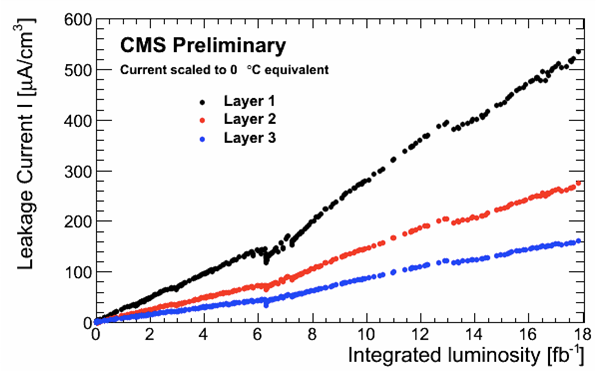
\includegraphics[width=0.45\textwidth]{\chfifteen/PixelLeakageCurrent.png}
 \end{center}
 \caption{Leakage current scaled to 0\unit{$^\circ$C} operational temperature for the barrel layers as a function of the integrated luminosity delivered in Run~1 representing the accumulated irradiation~\cite{Veszpremi:2014hpa}.}
 \label{fig:PixLeakageCurrent}
\end{figure}

The depletion voltage was also monitored during operations.
With irradiation, defects with a negative space charge are generated throughout the bulk leading to variations in the effective doping concentration.
When starting with $n$-type bulk, the effective doping concentration decreases because of the negatively charged defects until the bulk is transformed into an effective $p$-type.
This process, called type inversion, happens at a relatively low dose of several $10^{12}$\unit{$n_{eq}/cm^2$} (neutron equivalent fluence)~\cite{PixelDetectorsBook2006}.
As a consequence of this space charge sign inversion, the depletion zone now expands from the $n^+$-type pixel implants towards the p-type back.
The depletion voltage scales with the bulk doping concentration: it initially decreases reaching a minimum at the inversion point, and then rises with the effective bulk doping concentration.

A dedicated scan of the bias voltage was performed several times per year, by varying the detector bias voltage from 0\unit{V} to the the normal operating value of 150\unit{V} and measuring the single hit efficiency.
The results of the hit efficiency measurements for the innermost barrel layer between 2011 and the beginning of 2013 are shown in Fig.~\ref{fig:PixBiasV_a}.
%Figure~\ref{fig:PixRD_b} shows the results of hit efficiency measurements for Layer 1 of the barrel between 2011 and the beginning of 2013.
The bias voltage that is needed to reach a depletion depth corresponding to full hit efficiency decreases with irradiation at first, then increases as expected due to the aforementioned changes in the effective doping.
The dependence of the voltage needed to achieve full hit efficiency on the integrated luminosity is shown in Fig.~\ref{fig:PixBiasV_b} for the barrel layers and endcap disks.
The presence of a minimum for the layer 1 and layer 2 is evidence for type inversion occurrence.\\

\begin{figure}[!htb]
 \begin{center}
 \subfigure[]{\label{fig:PixBiasV_a}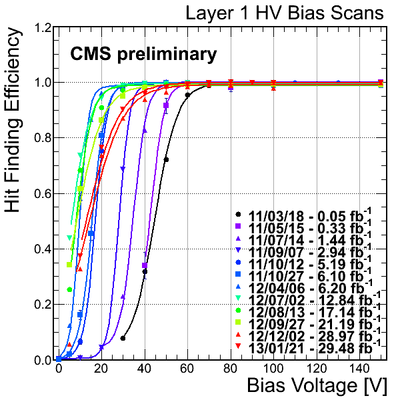
\includegraphics[width=0.45\textwidth]{\chfifteen/hv_l1_eff.png}}
 \subfigure[]{\label{fig:PixBiasV_b}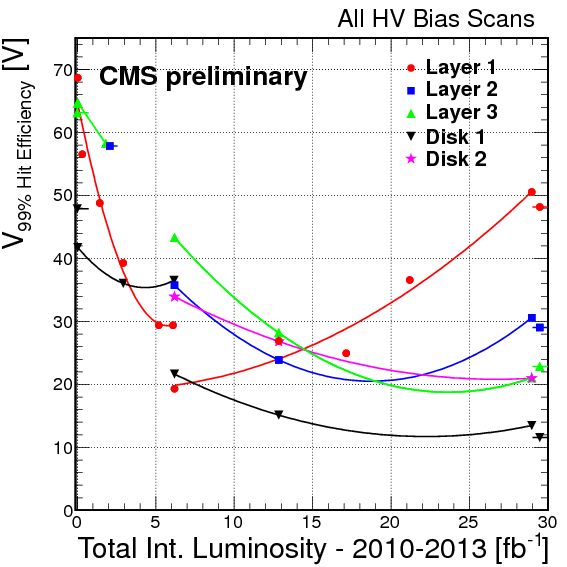
\includegraphics[width=0.45\textwidth]{\chfifteen/hvturnon_totlumi.png}}
 \end{center}
 \caption{(a) Scans of the bias voltage performed on the innermost barrel layer and (b) the bias voltage corresponding to full single hit efficiency for all barrel layers and forward disks as a function of the integrated luminosity delivered in Run~1~\cite{Veszpremi:2014hpa}.}
 \label{fig:PixBiasV}
\end{figure}

The evolution of the pixel thresholds and the analog currents was also frequently monitored in Run~1.
An increase of both pixel thresholds (Fig.~\ref{fig:PixRadDamag_a}) and analog currents (Fig.~\ref{fig:PixRadDamag_b}) was observed with integrated luminosity.
The possible explanation for these changes is the radiation damage in the bad-gap reference voltage circuit, which would shift all voltage settings inside the ROC.
The described effect required a re-calibration of the analog voltage and the pixels threshold during technical stops, in order to recover the optimal ROC performance.

The pixel hit resolution also exhibits a slow degradation with integrated luminosity as shown in Fig.~\ref{fig:PixRelvsLumi}. The two points of improvement correspond to re-calibrations of the pixel thresholds.

\begin{figure}[!htb]
 \begin{center}
 \subfigure[]{\label{fig:PixRadDamag_a}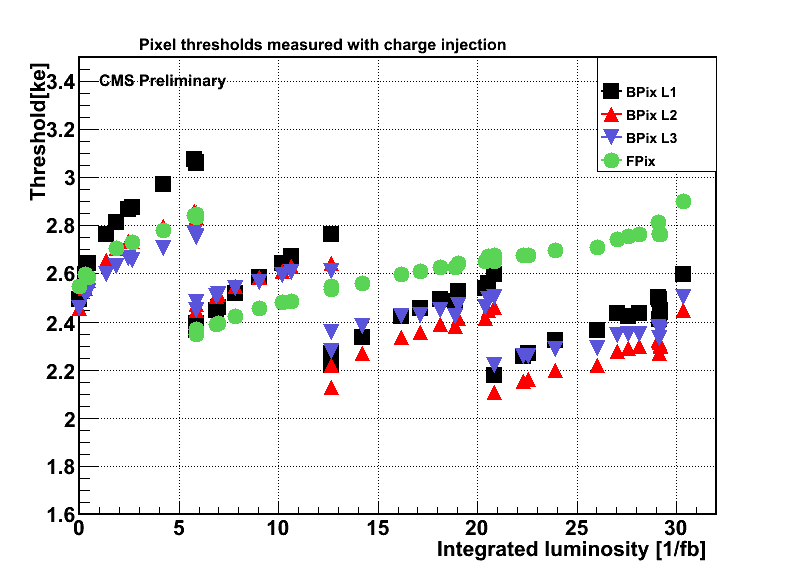
\includegraphics[width=0.45\textwidth]{\chfifteen/PixelThreshold_vs_IntLumi.png}}
 \subfigure[]{\label{fig:PixRadDamag_b}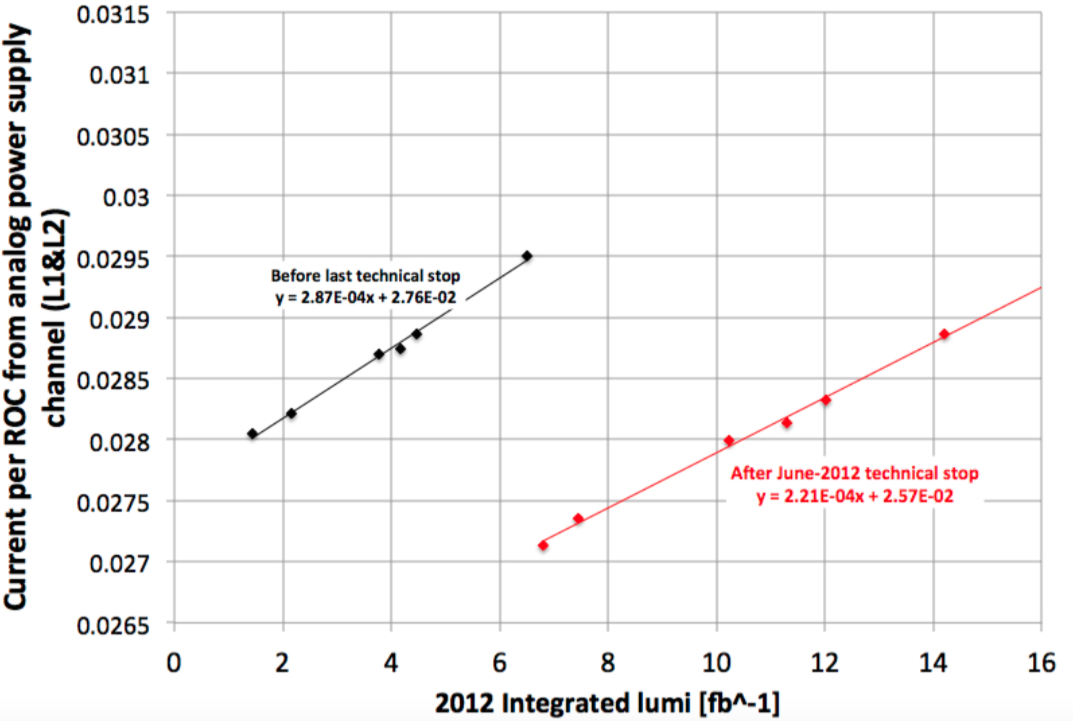
\includegraphics[width=0.45\textwidth]{\chfifteen/IanaROCvsLumi.png}}
 \end{center}
 \caption{(a) Average pixel thresholds in units of 1000 electrons for the barrel layers, and for the forward disks and (b) average analog current per ROC drawn by the power supply for BPix layers 1 and 2, as a function of the integrated luminosity delivered in Run~1~\cite{Veszpremi:2014hpa}.}
 \label{fig:PixRadDamag}
\end{figure}

\begin{figure}[!htb]
 \begin{center}
 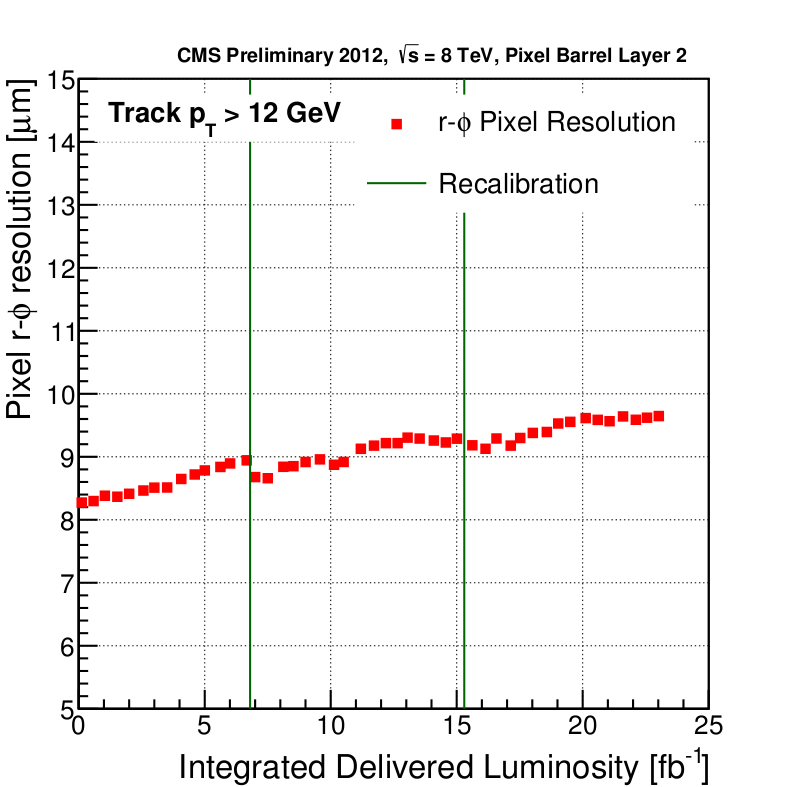
\includegraphics[width=0.45\textwidth]{\chfifteen/PixelResolutionL2_vs_IntLumi.png}
 \end{center}
 \caption{Single hit resolution for barrel layer 2 in the $r-\phi$ plane as a function of the integrated luminosity delivered in Run~1~\cite{Veszpremi:2014hpa}.}
 \label{fig:PixRelvsLumi}
\end{figure}

%%%%%%%%%%%
\section{Optimization for LHC Run 2}
%%%%%%%%%%%

\begin{wrapfigure}{R}{0.4\textwidth}
 \centering
 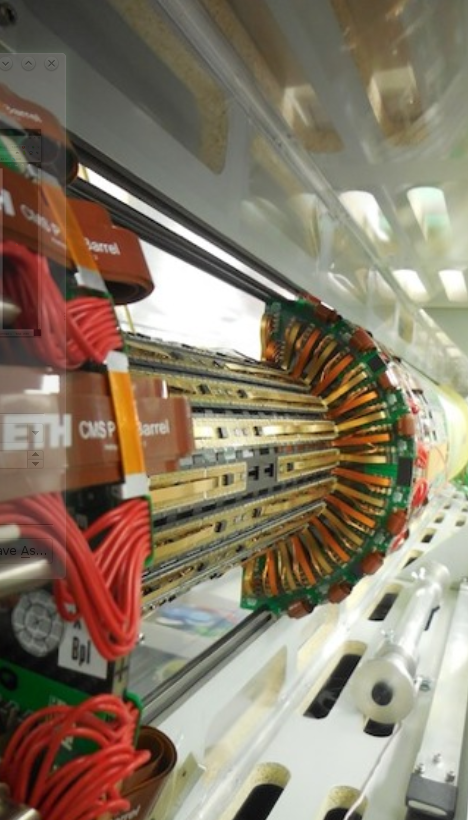
\includegraphics[width=0.35\textwidth]{\chfifteen/P5.png}
 \caption{Barrel pixel detector temporarily installed in P5.}
 \label{fig:PixP5}
\end{wrapfigure}

In summer 2013, after the first LHC run, the BPix and FPix detectors were extracted from CMS, and throughout LS1 they were kept in a refrigerated, climate-controlled room environment located at the CMS experimental site, P5.
The BPix was maintained in two cold boxes (Fig.~\ref{fig:PixP5}) in a lab with repair workbenches, and all the electronics and computers necessary to control and readout the detector for maintenance and tests.

At the end of Run~1, the fraction of operational channels in the barrel pixel detector was about 98\% and the long shutdown was used to recover the faulty channels.
The failure was mainly due to broken wire bond connections between ROCs and HDI. 
Replacements were attempted only for the barrel layer 3 outer shell, which made up 52\% of the faulty channels, since the other layers and the inner shell of layer 3 were considered too risky to touch without breaking further parts.
Two AOHs were found with disconnected wire bonds between the laser and the AOH PCB and they were also replaced. Figure~\ref{fig:AOHreplace} shows pictures from the lab in P5 during this operation. In order to proceed with the replacement one of the boxes was opened in order to take out the half shell of interest using a support equipped with rails. The shields covering the AOHs were opened and all the AOHs of the sector in the outside direction had to be unplugged in order to replace the two malfunctioning ones. Before closing again the detector inside the box, the two new AOHs were tested by checking with the oscilloscope the shift in the optical output baseline when changing the laser bias settings with commands sent through the tkFEC. The same tests were performed for the other functioning AOHs that had to be unplugged to perform the replacement. It was found that during the operation two additional AOHs had been broken and they had to be replaced as well.
In the end, the barrel pixel detector was about 99\% operational again.

There was, however, a serious incident in mid-August 2014. After having replaced a BPix module, tests of the corresponding quadrant showed severe damage: 55 modules were found to be not working anymore. It was decided to take that part of the detector to PSI for further tests and repairs. Shorts were discovered at the ROCs and in several modules between the TBM and cable pads. Eventually, the detector was repaired using 40 new modules and 19 repaired ones within three months. The shorts were suspected to be caused by humidity due to unobserved condensation in the cooling box. 
After being repaired, the functionalities of the new modules were successfully confirmed.

Part of the time available during LS1 have been employed to exercize and improve calibration procedures in view of re-commissioning and operation for Run~2.
An overview of the calibration procedure is given in the following.

\begin{figure}[!htb]
 \begin{center}
 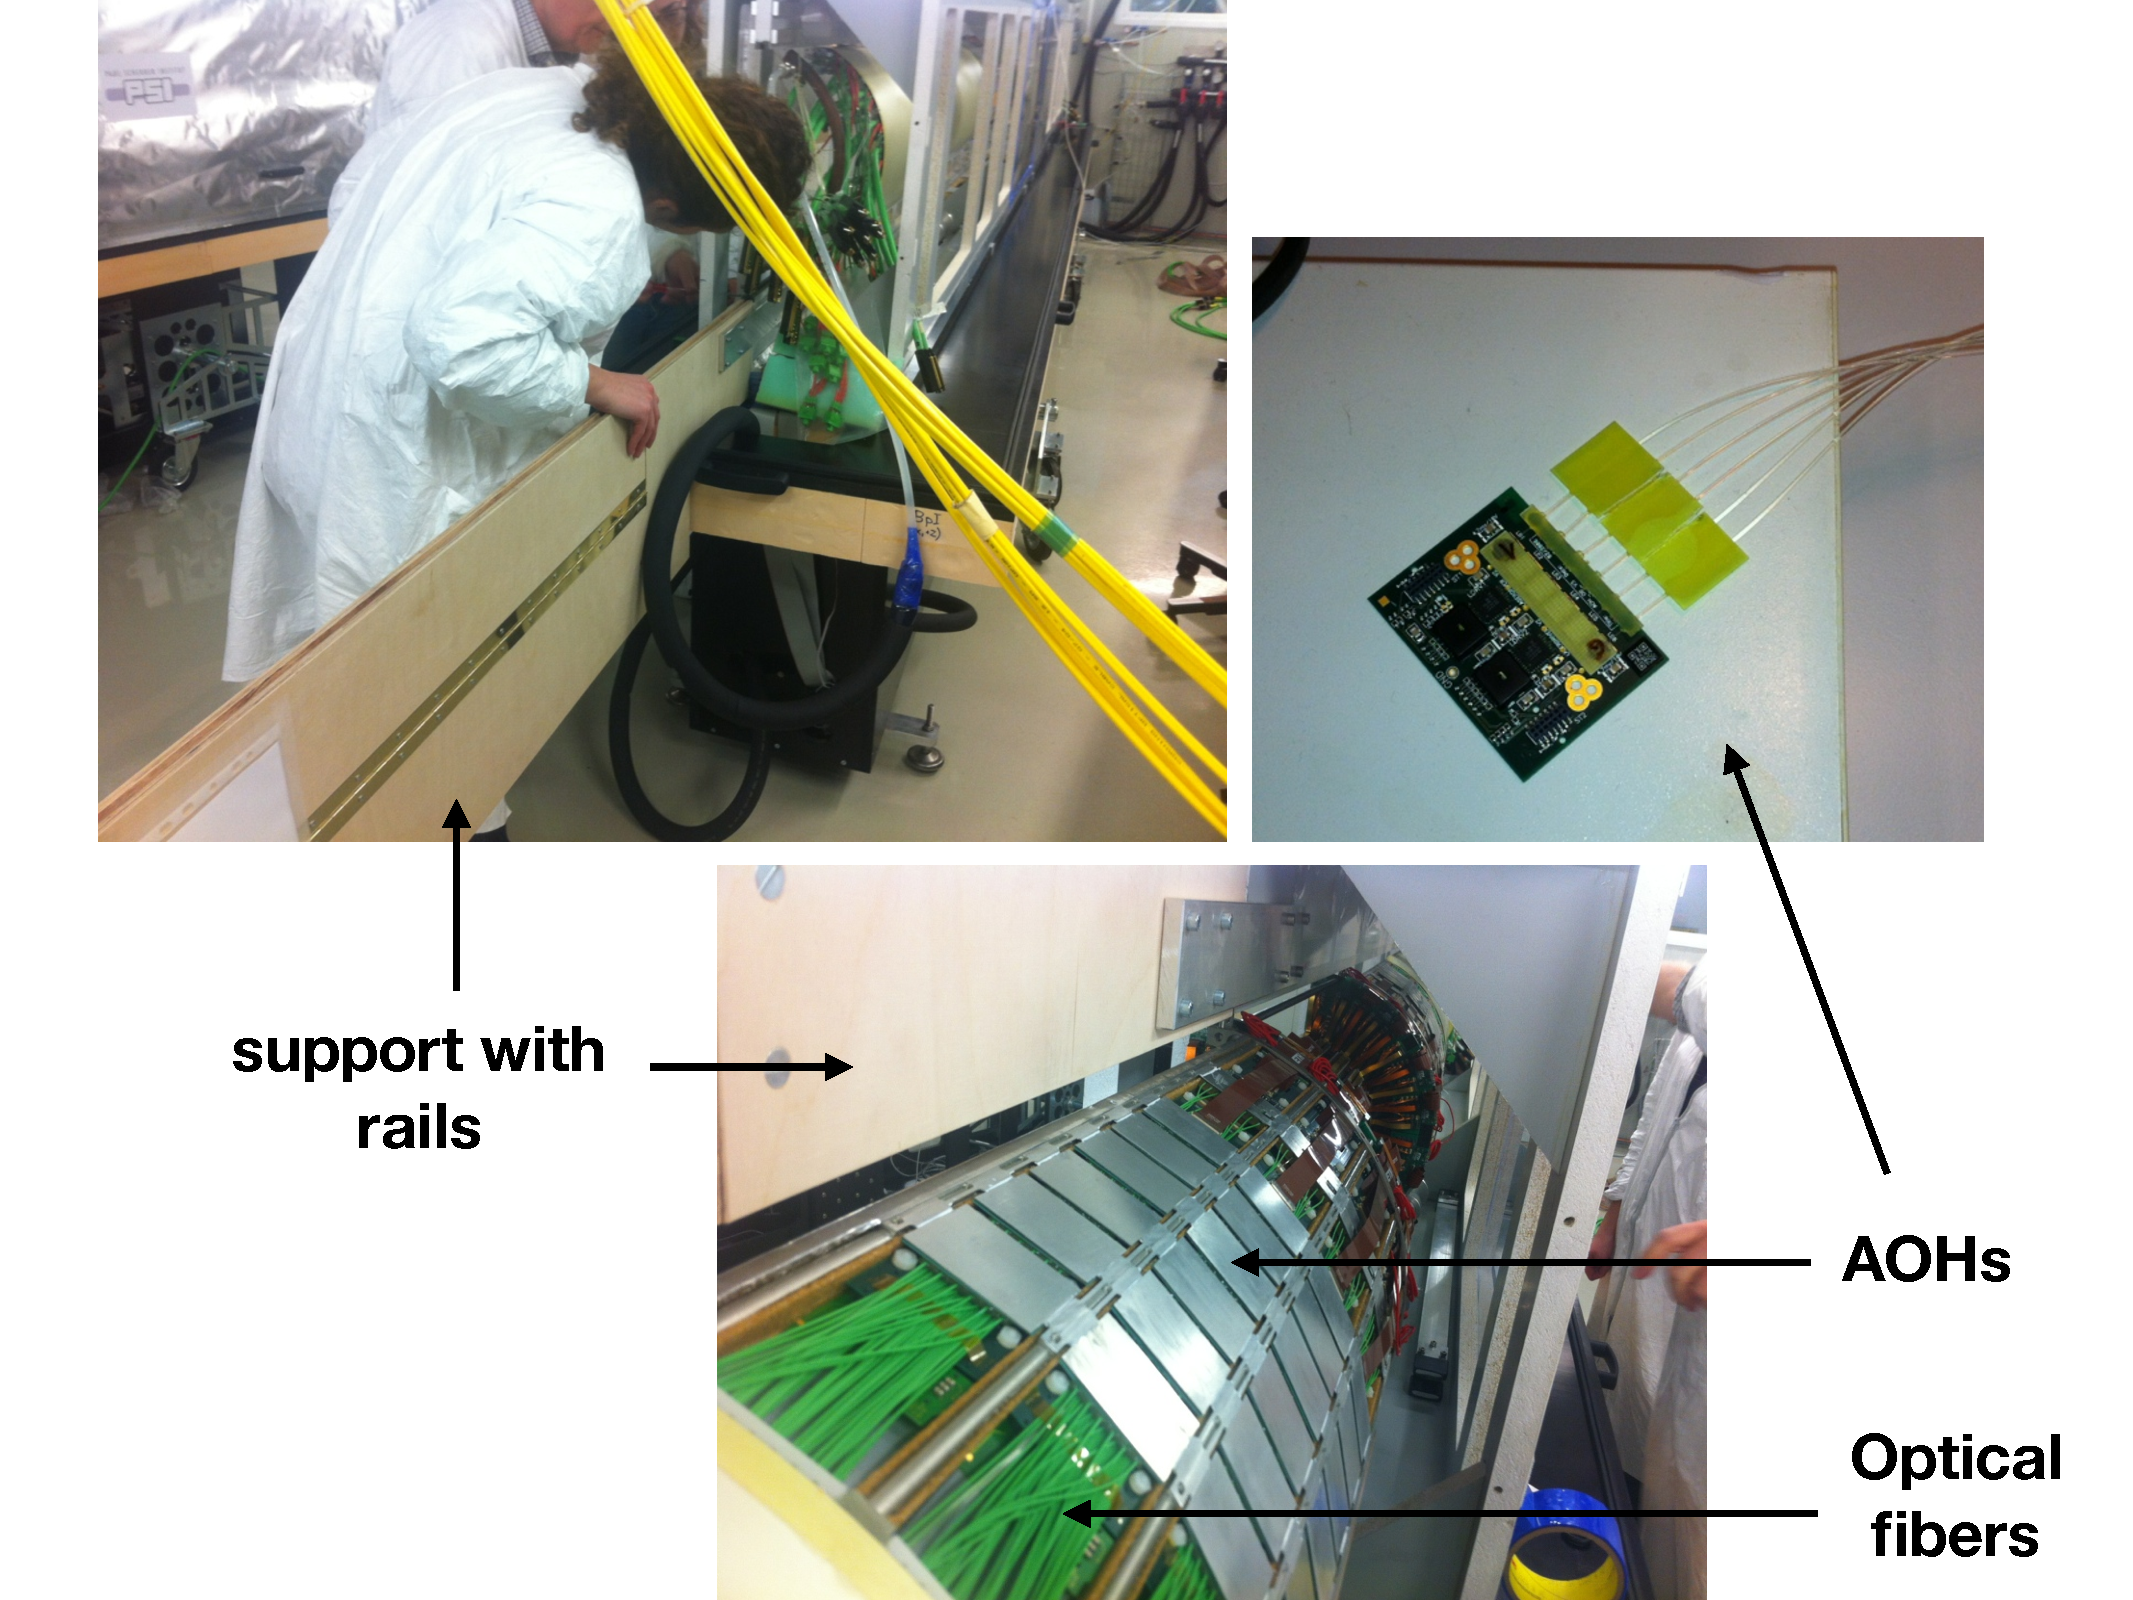
\includegraphics[width=0.7\textwidth]{\chfifteen/AOHReplacement.pdf}
 \end{center}
 \caption{blabla.}
 \label{fig:AOHreplace}
\end{figure}

%%%%%%%%%%%
\section{Overview of pixel calibrations}
%%%%%%%%%%%

Detector functioning and performance depend on proper calibrations of readout chain parameters.
Most of the readout parameters are quite stable unless major changes occur, such as the detector operating temperature.
Other parameters are more sensitive to environmental variations.
For these parameters a re-calibration on a regular basis was necessary during Run~1 operations.
Further expertise in the calibration procedure was achieved during LS1 and used 
for the re-commissioning of the detector to prepare it for a successful data-taking in 2015--2016.
In addition, the detector was fully re-calibrated at low temperature after re-installation.
As for Run~1, in these two years, re-calibrations have been performed during technical stops, and in particular in mid-2016 when the analog current drawn by the ROCs of the innermost layer reached critical values ($\sim 6$\unit{A}) that led to the trip of the power supplies in several occasions.
The calibrations were performed with POS which was installed and run on the computers available in the clean room.
As described in the following, there are a large number of different calibration tasks that need to be performed and sometimes iterated.

\subsection*{Delay25 chip}

\begin{figure}[!htb]
 \begin{center}
 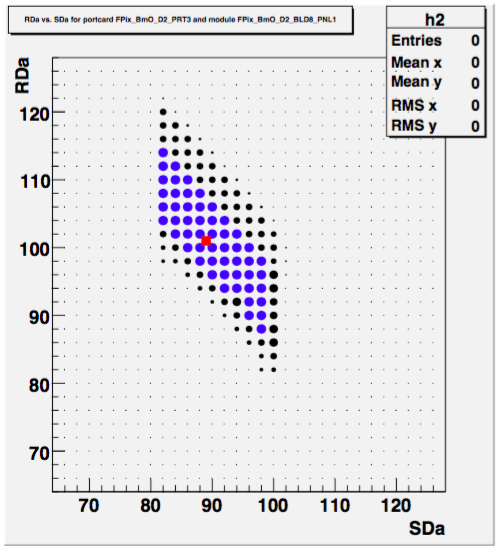
\includegraphics[width=0.45\textwidth]{\chfifteen/Delay25.png}
 \end{center}
 \caption{blabla.}
 \label{fig:Delay25}
\end{figure}

\subsection*{FED receiver offset}

%his calibration adjusts the input offset and channel offsets of the optical receivers in the FED such that the black level is adjusted to be near a given target value, normally 450, which is near the midpoint of the dynamic range of the ADC. During this calibration the baseline correction in the FED is turned off.
%Besides determining the input offset and the channel offsets the algorithm determines address levels for the black and ultra-black levels.
%The offset of the optical receiver in the FED needs to be adjusted to keep the baseline level of the signal in the middle of the ADC range.
%This baseline calibration is performed often because of its sensitivity to temperature variations. Automatic corrections are also applied to cope with minor temperature fluctuations.

\begin{figure}[!htb]
 \begin{center}
 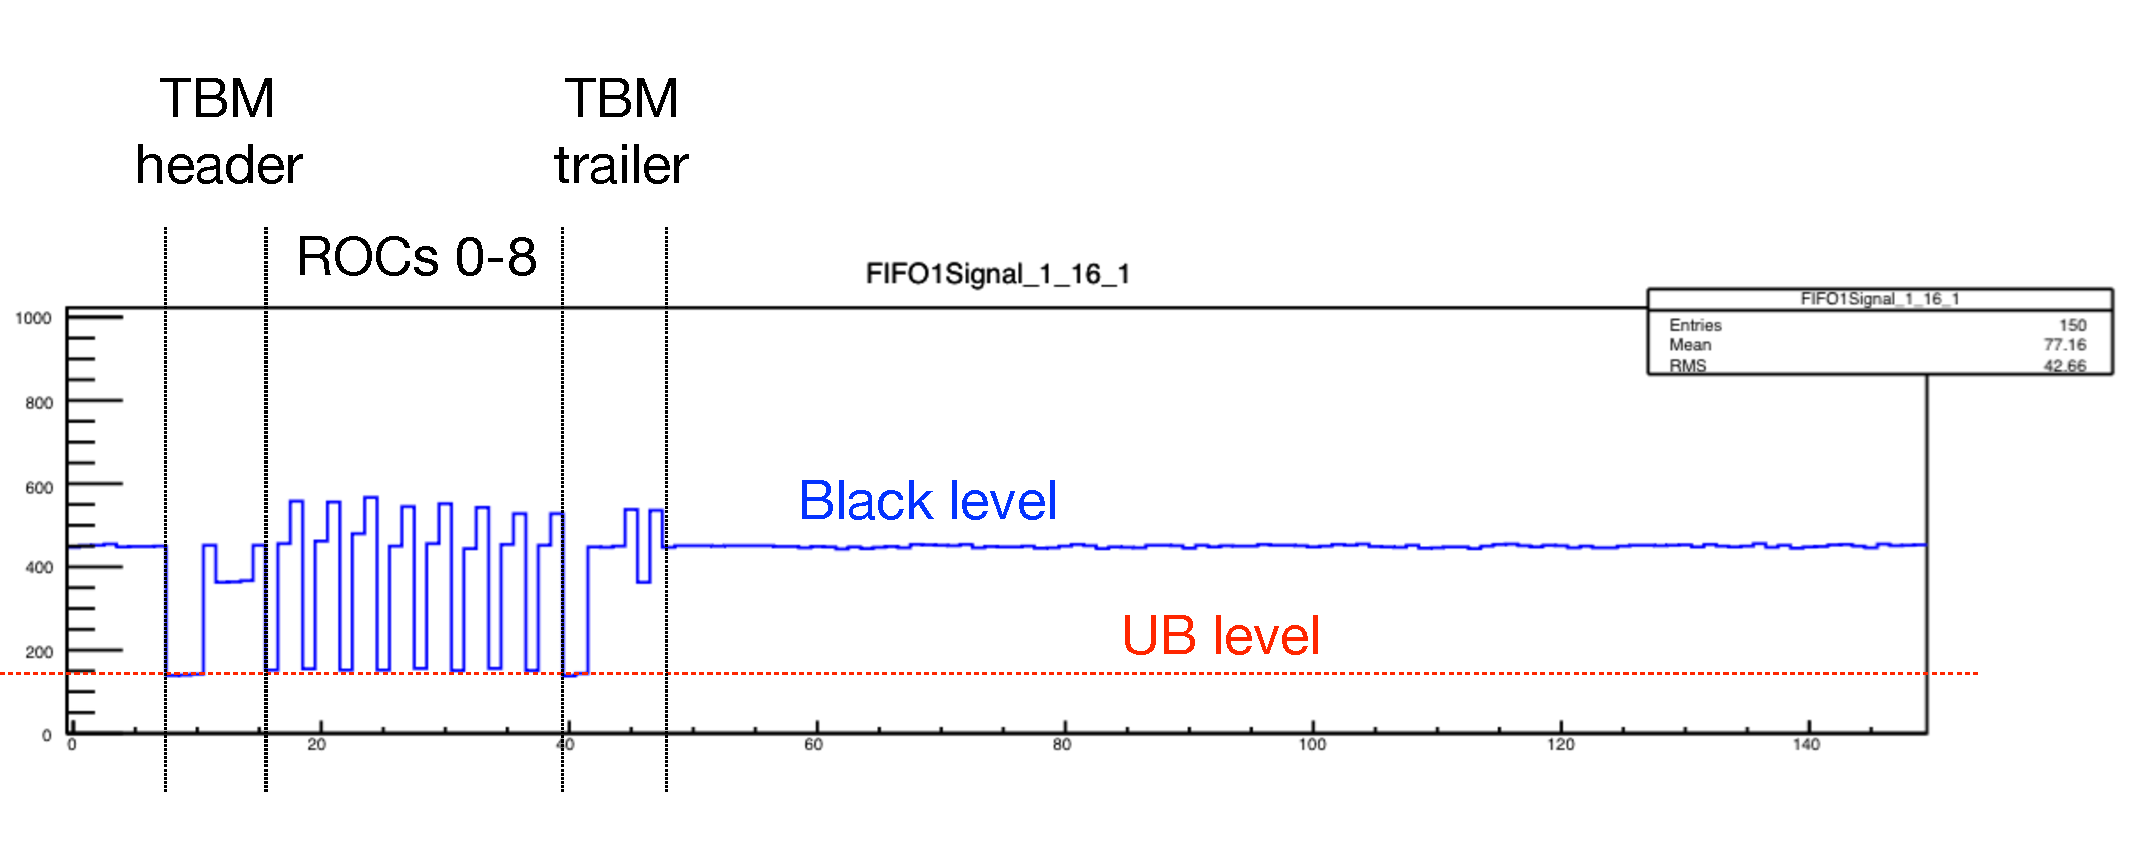
\includegraphics[width=0.45\textwidth]{\chfifteen/FEDBaseline.pdf}
 \end{center}
 \caption{blabla.}
 \label{fig:FEDBaseline}
\end{figure}

\subsection*{AOH bias and gain scan}

\begin{figure}[!htb]
 \begin{center}
 \includegraphics[width=0.45\textwidth]{\chfifteen/AOHBias.png}
 \end{center}
 \caption{blabla.}
 \label{fig:AOHBias}
\end{figure}

\subsection*{Clock phase}

\section{Re-commissioning for LHC Run 2}
\subsection{Installation into CMS}
\subsection{Check out of optical connections}
\subsection{Adjustment of readout chain settings}
\subsection{Optimisation of signal performance}